% This is samplepaper.tex, a sample chapter demonstrating the
% LLNCS macro package for Springer Computer Science proceedings;
% Version 2.21 of 2022/01/12
%
\documentclass[runningheads]{llncs}
%
\usepackage[T1]{fontenc}
% T1 fonts will be used to generate the final print and online PDFs,
% so please use T1 fonts in your manuscript whenever possible.
% Other font encondings may result in incorrect characters.
%
\usepackage{booktabs}
\usepackage{multirow}
\usepackage{amsmath,amssymb}
\usepackage{algorithm}
\usepackage{algpseudocode}
\usepackage{graphicx}
\usepackage{xspace}
\usepackage{pgfplots}
\usepackage{tikz}
\usepackage{hyperref}
\usepackage{array}

% If you use the hyperref package, please uncomment the following two lines
% to display URLs in blue roman font according to Springer's eBook style:
%\usepackage{color}
%\renewcommand\UrlFont{\color{blue}\rmfamily}
%\urlstyle{rm}
%
\begin{document}
%
\title{Noise-Gated Retrieval: Embedding-Based Context Compression for Cost-Aware RAG}
\titlerunning{Noise-Gated Retrieval for Cost-Aware RAG}
%
\author{First Author\inst{1}\orcidID{0000-1111-2222-3333} \and
Second Author\inst{2,3}\orcidID{1111-2222-3333-4444} \and
Third Author\inst{3}\orcidID{2222--3333-4444-5555}}
%
\authorrunning{F. Author et al.}
% First names are abbreviated in the running head.
% If there are more than two authors, 'et al.' is used.
%
\institute{Universidade de São Paulo, BR \and
Springer Heidelberg, Tiergartenstr. 17, 69121 Heidelberg, Germany
\email{lncs@springer.com}\\
\url{http://www.springer.com/gp/computer-science/lncs} \and
ABC Institute, Rupert-Karls-University Heidelberg, Heidelberg, Germany\\
\email{\{abc,lncs\}@uni-heidelberg.de}}
%
\maketitle              % typeset the header of the contribution
%
\begin{abstract}
Retrieval-augmented generation (RAG) commonly uses fixed top-$k$ retrieval despite its token cost. On HotpotQA distractor, fixed $k=10$ retrieval achieves strong F1 (0.792 on GPT-5.4-mini) but requires $\sim$14$\times$ more tokens than no retrieval (1452.5 vs 103.5 tokens). We systematically study five test-time context-compression strategies on this benchmark: fixed baselines ($k$=3, 5, 10), Adaptive-$k$ similarity-gap truncation, UCB1-TUNED rank-based bandit learning, LinUCB contextual bandit with lexical features, and a proposed noise-gate method combining cosine-similarity and Jaccard-overlap filtering.

On a matched sample of 400 HotpotQA distractor validation examples with GPT-5.4-mini, the noise gate with cosine threshold $\tau=0.3$ achieves F1=0.751 while reducing total tokens by 26.8\% relative to $k=10$ (1063.8 vs 1452.5 tokens)---remaining within ±0.05 F1 of the best lenient setting. In contrast, Adaptive-$k$ selects only $k^*=3.02$ documents on average but reaches only F1=0.627; UCB1-TUNED fails due to uniform gold-document rates across all rank positions (19.6--20.5\%), providing no exploitable signal; and LinUCB (F1=0.550 on gpt-5.4-mini) cannot distinguish semantically deceptive distractors using lexical features alone, underperforming fixed $k=3$ by 0.101 F1.

We demonstrate that the structural properties of distractor-heavy multi-hop QA---sparse and position-independent gold-document distribution, high-dimensional title non-stationarity, and semantic indistinguishability of distractors---make learned approaches fundamentally unsuitable for this problem class. Embedding-based threshold filtering is the minimal sufficient approach, achieving Pareto optimality at the quality--cost frontier.

\keywords{Retrieval-Augmented Generation \and Test-time Compression \and Context Filtering \and Noise Gating}
\end{abstract}

\section{Introduction}

Retrieval-augmented generation (RAG) improves language model performance on knowledge-intensive tasks by augmenting the model's parametric knowledge with relevant external documents~\cite{lewis2020rag}. In practice, most RAG systems use a simple fixed top-$k$ retrieval policy: retrieve the same number of documents for every query~\cite{klesel2025rag}. While straightforward to implement, this approach wastes tokens on every query that could be answered with fewer documents, and on low-utility documents within the retrieved set.

On HotpotQA distractor, a multi-hop question-answering benchmark where each example provides exactly 10 paragraphs (2 relevant, 8 distractors), this inefficiency is particularly acute. For GPT-5.4-mini, fixed $k=10$ retrieval achieves F1=0.792 but costs 1452.5 mean tokens per example---roughly $14\times$ the cost of answering without retrieval (103.5 tokens, F1=0.387). The research question is therefore: \emph{can we compress the retrieved context at inference time without significant quality loss?}

Three key properties of this benchmark make the question non-trivial. First, distractor paragraphs in HotpotQA are not random noise; they are retrieved by BM25 precisely because they are topically adjacent to the question, causing their embeddings to closely match those of true supporting facts. Second, HotpotQA's distractor split provides a fixed pool of 10 documents in a consistent BM25-determined order, making it a natural setting to study whether learned selection strategies can exploit this regularity. Third, multi-hop reasoning requires reasoning chains across multiple documents, so the problem is not merely to identify individually relevant passages but to select mutually complementary evidence sets.

We systematically evaluate five test-time context-compression strategies on 400 matched HotpotQA distractor validation examples: three fixed baselines ($k \in \{3, 5, 10\}$), Adaptive-$k$ similarity-gap truncation~\cite{taguchi2025adaptivek}, UCB1-TUNED rank-based bandit learning, LinUCB contextual bandit with lexical features, and a proposed noise-gate combining cosine and Jaccard filtering. The key empirical finding is that learned strategies underperform a simple threshold-based approach. We show this outcome is not a tuning artifact but rather a structural consequence of the benchmark's properties: uniform gold-document rates across rank positions (making rank-based bandits ineffective), pervasive title non-stationarity at inference time (making title-based bandits ineffective), and semantic indistinguishability of distractors (making lexical-feature bandits ineffective).

Our contributions are:
\begin{enumerate}
    \item \textbf{Systematic comparison} of five test-time context compression strategies on HotpotQA distractor ($n=400$, gpt-5.4-mini primary).
    \item \textbf{Noise-Gate method}: achieves $-26.8\%$ token reduction while staying within $\pm 0.05$ F1 of the $k=10$ baseline (F1=0.751 vs 0.792 at $\tau=0.3$, $\rho=0.65$).
    \item \textbf{Empirical analysis} explaining why Adaptive-$k$, UCB1-TUNED, and LinUCB fail due to structural properties of distractor-heavy multi-hop QA.
    \item \textbf{Ablation studies} across cosine threshold $\tau \in \{0.2, 0.25, 0.3, 0.35, 0.5\}$ and Jaccard threshold $\rho \in \{0.50, 0.55, 0.65\}$.
\end{enumerate}

\section{Related Work}

This work sits at the intersection of four research areas. Table~\ref{tab:related_positioning} summarizes the positioning.

\begin{table}[t]
\small
\begin{tabular}{>{\raggedright\arraybackslash}p{2.5cm}
                >{\raggedright\arraybackslash}p{4.5cm}
                >{\raggedright\arraybackslash}p{4cm}}
\toprule
\multicolumn{1}{c}{\textbf{Area}} &
\multicolumn{1}{c}{\textbf{Representative Works}} &
\multicolumn{1}{c}{\textbf{How We Differ}} \\
\midrule
\textbf{Fixed-Budget RAG} & Lewis et al. (RAG), Klesel \& Wittmann, Zhao et al. & We study compression of a fixed retrieved pool, not pipeline design \\
\midrule
\textbf{Adaptive Retrieval} & Self-RAG, DioR, DRAGIN & We filter \emph{what was retrieved}, not decide \emph{whether to retrieve} \\
\midrule
\textbf{Context Noise Compression} & SetR, ReflectiveRAG, Adaptive-$k$ & We use threshold-based filtering; others use set-level or gap-based selection \\
\midrule
\textbf{Bandit/RL for IR} & UCB, Thompson Sampling, contextual bandits & We show bandits fundamentally fail on this problem class and explain why \\
\bottomrule
\end{tabular}
\label{tab:related_positioning}
\end{table}

\paragraph{Fixed-budget retrieval.}
Foundational RAG systems retrieve the top-$k$ documents by relevance~\cite{lewis2020rag}. Fixed $k$ remains the dominant approach in deployed systems~\cite{klesel2025rag}. Our work takes fixed $k=10$ retrieval as the quality baseline and asks how to retain its quality at lower token cost.

\paragraph{Adaptive retrieval control.}
Self-RAG~\cite{asai2024selfrag}, DioR~\cite{guo2025dior}, and DRAGIN~\cite{su2024dragin} learn when to retrieve and how much to retrieve using training or learned tokens. These methods require additional training or model modification. Our work is orthogonal: we focus on filtering a fixed retrieved pool without training, a test-time-only strategy.

\paragraph{Context noise and compression.}
Adaptive-$k$~\cite{taguchi2025adaptivek} selects documents by similarity-score gaps. SetR~\cite{lee2025setr} and RankRAG~\cite{yu2024rankrag} select context as a set using complementarity and downstream usefulness. ReflectiveRAG~\cite{verma2026reflectiverag} shows that irrelevant or redundant context can hurt quality. Our noise-gate component is conceptually related to Maximum Marginal Relevance~\cite{goldstein1998mmr}, which trades off relevance and diversity, but uses a simpler two-stage design: cosine similarity for relevance, Jaccard overlap for redundancy.

\paragraph{Bandits and learning-to-rank.}
Bandit algorithms (UCB, Thompson Sampling, contextual bandits with LinUCB) have been applied to retrieval, ranking, and exploration-exploitation problems broadly. We test whether UCB1-TUNED and LinUCB can learn useful context-selection signals on HotpotQA distractor, finding they cannot due to structural properties of the benchmark. This is a contribution in itself: we identify and explain failure modes in a concrete setting.

\section{Problem Formulation}

Given a question $q$ and a fixed pool of retrieved documents $D = \{d_1, d_2, \ldots, d_{10}\}$ (obtained via BM25 or similar), we seek a subset $S^* \subseteq D$ that maximizes answer quality while minimizing token cost. Formally,
\[
S^* = \arg\max_{S \subseteq D} \left[ F_1(\text{answer} \mid q, S) - \lambda \cdot |{\text{tokens}(S)}| \right],
\]
where $F_1$ is the token-level F1 score against the gold answer, $|{\text{tokens}(S)}|$ is the total input tokens required to encode $q$ and $S$, and $\lambda$ is a cost weight.

This formulation scopes the problem: we do not control whether to retrieve (that decision is fixed as ``retrieve the top 10''), nor do we control the retrieval algorithm itself (BM25 order is fixed). We only control what subset $S$ of the retrieved documents to pass to the model.

We report three metrics: token-level F1 score (primary), exact match (EM, secondary), and mean total tokens per question (cost metric).

\section{Methods}

We explore the design space of test-time context compression via five strategies, spanning learned and threshold-based approaches along two axes: question-level vs.\ section-level control, and training-free vs.\ training-required methods.

\subsection{Baselines}

\begin{itemize}
    \item \textbf{always\_think}: Answer directly with no retrieval (103--132 mean tokens, F1=0.387--0.441 across models).
    \item \textbf{retrieval\_k3}: Top-3 retrieved documents (465--516 tokens, F1=0.588--0.681).
    \item \textbf{retrieval\_k5}: Top-5 retrieved documents (726--809 tokens, F1=0.632--0.727).
    \item \textbf{retrieval\_k10}: All 10 retrieved documents (1447--1640 tokens, F1=0.707--0.792).
\end{itemize}

\subsection{Adaptive-$k$ (Similarity-Gap Truncation)}

Given retrieved documents with similarity scores $s_1 \ge s_2 \ge \cdots \ge s_{10}$, Adaptive-$k$~\cite{taguchi2025adaptivek} selects a cut point via the largest adjacent gap:
\begin{equation}
k^* = \arg\max_{1 \le i < 10} (s_i - s_{i+1}).
\end{equation}
This selects a compact cluster of high-confidence documents. However, in HotpotQA distractor, distractors are drawn to be topically adjacent to the gold evidence, causing their embedding scores to closely match true supporting facts. The largest gap often falls within a cluster of similar distractors rather than cleanly separating signal from noise.

\subsection{UCB1-TUNED (Rank-Based Bandit)}

We test whether a bandit algorithm can learn which rank positions are historically valuable. Using Welford online statistics over the full training split ($n=90,447$ HotpotQA distractor examples), we track mean reward and variance for each rank position (0--9). Binary reward is assigned: 1.0 if the paragraph at that rank contains a supporting fact, else 0.0. At inference, each position is scored via standard UCB1-TUNED:
\[
\mathrm{score}(\text{rank}) = \mu_{\text{rank}} + \sqrt{\frac{\ln T}{n_{\text{rank}}} \cdot \min(0.25, \sigma_{\text{rank}}^2)}.
\]
The reranker then selects the top-$k$ positions by this score.

\subsection{LinUCB (Contextual Bandit with Lexical Features)}

This variant learns per-document reward estimates using ridge regression with three lexical features: (1) token overlap between question and section, (2) title-in-question fraction, and (3) section token length. A UCB bonus is added for exploration. Unlike rank-based UCB, this approach attempts to learn document-level utility directly.

\subsection{Noise-Gate (Two-Stage Embedding Filter)}
\label{sec:methods_noisegate}

This method applies two complementary filters at inference time with no training.

\textbf{Stage 1 (Cosine filter):} Remove paragraphs whose cosine similarity to the question falls below threshold $\tau$:
\begin{equation}
\mathrm{cos}(q, d_i) = \frac{e_q \cdot e_i}{\|e_q\| \, \|e_i\|} \ge \tau.
\end{equation}

\textbf{Stage 2 (Jaccard filter):} Among paragraphs surviving Stage 1, remove those whose word-overlap with already-kept paragraphs exceeds threshold $\rho$:
\begin{equation}
\max_{d_j \in \text{kept}} \frac{|d_i \cap d_j|}{|d_i \cup d_j|} \le \rho.
\end{equation}

We evaluate $\tau \in \{0.2, 0.25, 0.3, 0.35, 0.5\}$ and $\rho \in \{0.50, 0.55, 0.65\}$. Embeddings are computed using multi-qa-MiniLM-L6-cos-v1 (dimension 384, pre-trained on diverse QA corpora).

\section{Experiments}
\label{sec:experiments}

\subsection{Setup}

\textbf{Dataset.}
We evaluate on HotpotQA~\cite{yang2018hotpotqa}, distractor subset, validation split. Each example contains exactly 10 paragraphs: 2 supporting facts and 8 distractors retrieved by BM25 to be topically adjacent to the question. We use a fixed random sample of $n{=}400$ examples for all experiments, large enough to stabilize mean F1 and EM while remaining practical for matched-sample ablations.

\textbf{Model.}
All experiments use \texttt{gpt-5.4-mini} as the single generation model. Fixing the model eliminates confounds from tokenization, pricing, and provider-specific prompting behavior, and focuses the comparison on context-selection strategy alone.

\textbf{Metrics.}
We report token-level F1 (primary), exact match (EM), and mean total tokens per example. F1 measures answer quality; total tokens measure the cost of the context passed to the model. We define a practical tolerance of $\pm 0.05$~F1 relative to the $k{=}10$ baseline: strategies within this band are considered quality-preserving.

\textbf{Baselines.}
We compare against three fixed retrieval policies:
\begin{itemize}
    \item \textbf{No retrieval} ($k{=}0$): the model answers from parametric knowledge only.
    \item \textbf{Fixed $k{=}5$}: the top-5 BM25-ranked paragraphs are passed as context.
    \item \textbf{Fixed $k{=}10$}: all 10 paragraphs are passed (quality upper bound).
\end{itemize}

\textbf{Strategies under evaluation.}
In addition to the baselines, we evaluate four context-compression strategies, all operating on the same fixed pool of 10 retrieved paragraphs:
\begin{itemize}
    \item \textbf{Adaptive-$k$}: a CART decision tree trained to predict the optimal $k \in [1,9]$ from question features; selects the top-$k^*$ paragraphs by embedding similarity.
    \item \textbf{UCB1-TUNED}: a title-based bandit reranker that tracks per-title reward statistics over the training split and selects the top-$k$ titles by UCB score at inference. Unseen titles fall back to BM25 ranking.
    \item \textbf{LinUCB}: a contextual bandit that uses lexical features (token overlap, title-in-question fraction, section length) and ridge-regression reward estimation with an exploration bonus.
    \item \textbf{Noise-Gate} (proposed): the two-stage filter from Section~\ref{sec:methods_noisegate}. No training required.
\end{itemize}
For the bandit strategies (UCB1-TUNED and LinUCB), we report results at $k{=}5$ to allow direct comparison with the fixed $k{=}5$ baseline at equal retrieval budget.

\subsection{Main Results}
\label{subsec:main_results}

Table~\ref{tab:main_results} presents the unified comparison across all strategies. The fixed $k{=}10$ baseline achieves F1~0.792 with 1452.5 mean total tokens, confirming that full retrieval is a strong quality reference but an expensive one: it uses $14\times$ more tokens than no retrieval ($k{=}0$, 103.5 tokens).

Among the compression strategies, Noise-Gate at $\tau{=}0.3$ achieves the best quality--cost tradeoff: F1~0.751 with 1063.8 tokens, a 26.7\% token reduction while remaining within the $\pm 0.05$ F1 tolerance of the $k{=}10$ baseline. Noise-Gate at $\tau{=}0.2$ preserves even more quality (F1~0.774) with a modest 9.3\% saving.

The learned strategies fail to match even the fixed $k{=}5$ baseline at equal budget. UCB1-TUNED at $k{=}5$ reaches F1~0.704 with 723 tokens---superficially close to fixed $k{=}5$ (0.716, 732 tokens)---but this similarity is misleading: 83.8\% of validation titles are unseen in training, so UCB1 falls back to BM25 ranking on the vast majority of queries. Its apparent competitiveness reflects BM25 performance, not learned selection. LinUCB at $k{=}5$ performs worse still (F1~0.620, 686 tokens), confirming that lexical features alone cannot distinguish distractors from supporting facts. Adaptive-$k$ selects compact contexts (mean $k^*{=}3.02$, 483 tokens) but its F1~0.627 falls below fixed $k{=}5$.

%% NOTE: Figure 1 (F1 vs Tokens Pareto scatter) to be placed here once generated.
%% \begin{figure}[t]
%%     \centering
%%     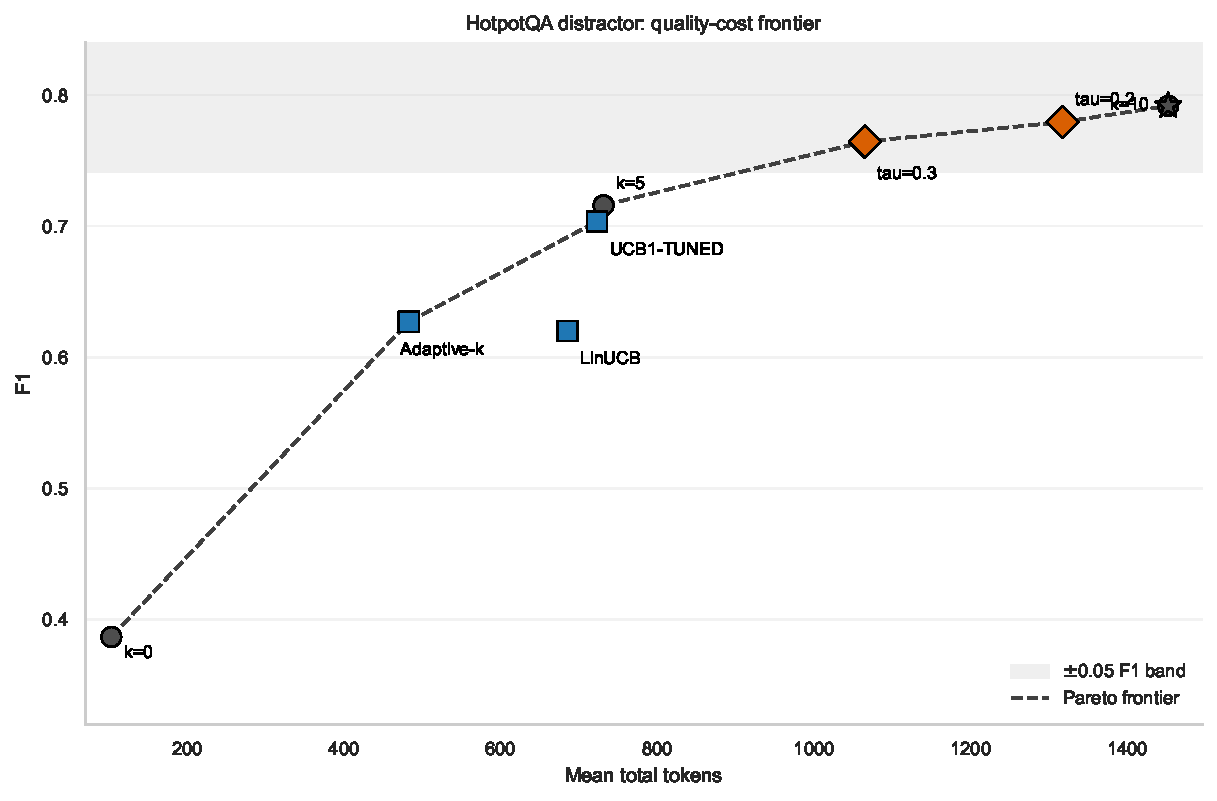
\includegraphics[width=\linewidth]{images/pareto_f1_vs_tokens.pdf}
%%     \caption{F1 vs.\ mean total tokens for all strategies. The Pareto frontier (dashed) shows that Noise-Gate $\tau{=}0.3$ is the knee of the curve: it offers the largest token savings within the $\pm 0.05$ F1 tolerance band (shaded).}
%%     \label{fig:pareto}
%% \end{figure}

\begin{table*}[t]
\centering
\caption{Main results on \texttt{gpt-5.4-mini} (HotpotQA distractor validation, $n{=}400$). Strategies are grouped by type. ``Savings'' is the token reduction relative to fixed $k{=}10$. ``In range'' indicates whether F1 is within $\pm 0.05$ of the $k{=}10$ reference (0.792).}
\label{tab:main_results}
\begin{tabular}{llrrrrl}
\toprule
Type & Strategy & F1 & EM & Tokens & Savings & In range? \\
\midrule
\multirow{3}{*}{Baselines}
& No retrieval ($k{=}0$)  & 0.387 & 0.278 & 103.5  & $-$92.9\% & \texttimes \\
& Fixed $k{=}5$           & 0.716 & 0.555 & 731.7  & $-$49.6\% & \texttimes \\
& Fixed $k{=}10$          & 0.792 & 0.632 & 1452.5 & ---       & ref. \\
\midrule
\multirow{3}{*}{Learned}
& Adaptive-$k$ (CART)     & 0.627 & 0.475 & 483.1  & $-$66.8\% & \texttimes \\
& UCB1-TUNED ($k{=}5$)    & 0.704 & 0.570 & 723.0  & $-$50.2\% & \texttimes \\
& LinUCB ($k{=}5$)        & 0.620 & 0.489 & 686.0  & $-$52.8\% & \texttimes \\
\midrule
\multirow{2}{*}{Noise-Gate}
& $\tau{=}0.2$            & 0.774 & 0.620 & 1317.5 & $-$9.3\%  & \checkmark \\
& $\tau{=}0.3$            & 0.751 & 0.598 & 1063.8 & $-$26.7\% & \checkmark \\
\bottomrule
\end{tabular}
\end{table*}

\subsection{Noise-Gate Threshold Ablation}
\label{subsec:tau_ablation}

To map the full quality--cost frontier of the noise gate, we sweep the cosine threshold $\tau \in \{0.2, 0.25, 0.3, 0.35, 0.5\}$ at fixed Jaccard redundancy threshold $\rho{=}0.65$. Table~\ref{tab:noise_gate_thresholds} reports the results.

%% TODO: Fill in τ=0.25 and τ=0.35 rows once experiment completes.

\begin{table}[t]
\centering
\caption{Noise-gate $\tau$ sweep on \texttt{gpt-5.4-mini} ($\rho{=}0.65$, $n{=}400$). Rows ordered by increasing $\tau$. Bold marks the recommended operating point.}
\label{tab:noise_gate_thresholds}
\begin{tabular}{rrrrrr}
\toprule
$\tau$ & F1 & EM & Tokens & Savings & In range? \\
\midrule
0.20 & 0.774 & 0.620 & 1317.5 & $-$9.3\%  & \checkmark \\
0.25 & ---   & ---   & ---    & ---       & --- \\
\textbf{0.30} & \textbf{0.751} & \textbf{0.598} & \textbf{1063.8} & $-$\textbf{26.7\%} & \checkmark \\
0.35 & ---   & ---   & ---    & ---       & --- \\
0.50 & 0.613 & 0.480 & 403.9  & $-$72.2\% & \texttimes \\
\bottomrule
\end{tabular}
\end{table}

The sweep reveals a clear monotonic tradeoff: as $\tau$ increases, both F1 and token usage decrease. The lenient setting ($\tau{=}0.2$) preserves the most quality (F1~0.774) but saves only 9.3\% of tokens. The strict setting ($\tau{=}0.5$) achieves dramatic savings ($-$72.2\%) but drops F1 to 0.613, well outside the tolerance band. The recommended operating point $\tau{=}0.3$ sits at the knee: it offers meaningful savings ($-$26.7\%) while staying within the $\pm 0.05$ F1 tolerance. Output tokens remain nearly constant across thresholds ($\approx$6.7), confirming that savings come entirely from reduced input context.

%% NOTE: Figure 2 (τ ablation line chart, dual y-axis F1 and Tokens) to be placed here once generated.

\subsection{Jaccard Redundancy Ablation}
\label{subsec:rho_ablation}

Table~\ref{tab:noise_gate_jaccard_ablation} ablates the Jaccard redundancy threshold $\rho \in \{0.50, 0.55, 0.65\}$ across three cosine thresholds. The redundancy parameter has a small effect: at $\tau{=}0.2$, F1 ranges from 0.774 to 0.782 across all $\rho$ values, a spread of only 0.008. At $\tau{=}0.3$ the spread is 0.011, and at $\tau{=}0.5$ it is 0.024. Token usage is similarly stable: at $\tau{=}0.3$, mean tokens vary by fewer than 10 across $\rho$ settings.

The best absolute F1 in this grid is 0.782 at $(\tau{=}0.2, \rho{=}0.50)$, but the gain over the default $\rho{=}0.65$ is marginal ($+$0.008~F1) and comes with no meaningful token difference. This confirms that the cosine threshold $\tau$ is the dominant control: it determines the quality--cost operating point, while the Jaccard threshold $\rho$ acts as a secondary refinement with limited sensitivity.

\begin{table*}[t]
\centering
\caption{Jaccard redundancy ablation on \texttt{gpt-5.4-mini} ($n{=}400$). Each cell shows F1 / mean total tokens for the $(\tau, \rho)$ combination.}
\label{tab:noise_gate_jaccard_ablation}
\begin{tabular}{lrrrrrr}
\toprule
& \multicolumn{3}{c}{F1} & \multicolumn{3}{c}{Total Tokens (mean)} \\
\cmidrule(lr){2-4}\cmidrule(lr){5-7}
Jaccard $\rho$ & $\tau{=}0.2$ & $\tau{=}0.3$ & $\tau{=}0.5$ & $\tau{=}0.2$ & $\tau{=}0.3$ & $\tau{=}0.5$ \\
\midrule
0.50 & 0.782 & 0.759 & 0.626 & 1308.0 & 1055.6 & 401.6 \\
0.55 & 0.781 & 0.748 & 0.602 & 1309.6 & 1057.3 & 401.8 \\
0.65 & 0.774 & 0.751 & 0.613 & 1317.5 & 1063.8 & 403.9 \\
\bottomrule
\end{tabular}
\end{table*}

\section{Analysis: Why Learned Methods Fail on Distractor-Heavy Multi-Hop QA}
\label{sec:analysis}

We tested three learned context-selection strategies on HotpotQA distractor: Adaptive-$k$, UCB1-TUNED (over both rank positions and paragraph titles), and LinUCB with lexical features. In every head-to-head comparison, a zero-training noise gate matches or exceeds them. In this section we argue that this outcome is not a tuning artifact but a structural consequence of three dataset-level properties: deceptive topicality of distractors, non-stationarity of arm identity, and lexical confusability between distractors and gold paragraphs. Sections~\ref{subsec:fail_adaptivek}--\ref{subsec:fail_linucb} identify why each learned strategy fails, and \S\ref{subsec:why_noise_gate} explains why a single deterministic embedding threshold sidesteps all three failure modes at once.

\subsection{Adaptive-$k$: similarity gaps place the cut in the wrong cluster}
\label{subsec:fail_adaptivek}

The Adaptive-$k$ rule truncates the retrieved list at the largest adjacent similarity gap~\cite{taguchi2025adaptivek}, under the implicit assumption that embedding-similarity rank is monotone in true relevance. Our main results in Table~\ref{tab:main_results} show that in HotpotQA distractor this assumption is too weak to be useful. Adaptive-$k$ selects compact contexts (mean $k^*=3.02$, mean total tokens 483.1) but reaches only F1 0.627, below even fixed \texttt{retrieval\_k3} (0.651), \texttt{retrieval\_k5} (0.716), and \texttt{retrieval\_k10} (0.792). It uses fewer tokens, but loses answer quality faster than tokens.

The mechanism is dataset-specific. HotpotQA distractors are drawn by BM25 to be topically adjacent to the gold evidence: they share entities, vocabulary, and discourse style with the question. This pushes their embedding-similarity scores close to, and in some cases above, those of the true supporting facts. When the gap rule scans this score sequence, the ``largest gap'' frequently lies inside a cluster of topically similar distractors rather than cleanly separating supporting facts from noise. Selecting the top-$k^*$ paragraphs then excludes genuine evidence while retaining topical but unhelpful context. In other words, Adaptive-$k$ does not fail because it keeps too few paragraphs; it fails because the few it keeps are the wrong ones.

\subsection{UCB1-TUNED: rank positions and titles are both non-stationary arms}
\label{subsec:fail_ucb1}

We explored whether a bandit reranker could learn which retrieved items are historically valuable. Two natural arm definitions are available: rank positions (0--9 in BM25 order) and paragraph titles. Both fail, for related but distinct reasons.

\paragraph{Rank positions carry no signal.}
Table~\ref{tab:ucb1_rank_results} already reported the rank-based variant on \texttt{gpt-4o-mini}: F1 is 0.300 at $k=2$, 0.347 at $k=3$, and 0.414 at $k=5$, all well below the matching fixed baselines. The reason is structural. In the full training split ($n=90{,}447$), the gold rate across rank positions is nearly uniform: rank 0 contains a supporting fact 20.45\% of the time, rank 9 contains one 19.60\% of the time, and intermediate ranks fall inside this narrow band. There is therefore no persistent ``good rank'' to exploit. A UCB1 reranker operating over rank positions reduces to exploration noise plus an additive constant, because BM25's ordering over HotpotQA distractor paragraphs does not encode supporting-fact containment.

\paragraph{Title identity is non-stationary across queries.}
A more refined variant treats paragraph titles as arms. Table~\ref{tab:ucb1_title_coldstart} reports the cold-start behavior of this variant on \texttt{gpt-5.4-mini} with matched samples of $n=400$ per $k$. At $k=5$, $83.8\%$ of validation queries touch titles that were never observed during training. For those queries the learned reward estimates $\hat Q(\text{title})$ are undefined and the reranker silently falls back to BM25---precisely the policy it was meant to improve. At $k=2$ and $k=3$, cold-start rates are $61.5\%$ and $75.2\%$ respectively: still a large majority of queries for which no learned signal exists.

\begin{table}[t]
\centering
\caption{Title-based UCB1-TUNED cold-start rates on \texttt{gpt-5.4-mini} ($n=400$ matched samples per $k$). A cold-start query is one whose selected titles were not observed during training, triggering a BM25 fallback.}
\label{tab:ucb1_title_coldstart}
\begin{tabular}{lrrr}
\toprule
$k$ & Samples & Unseen titles & Cold-start \% \\
\midrule
2 & 400 & 246 & 61.5 \\
3 & 400 & 301 & 75.2 \\
5 & 400 & 335 & 83.8 \\
\bottomrule
\end{tabular}
\end{table}

The resulting quality reflects this: overall F1 aggregated across $k\in\{2,3,5\}$ is 0.623, and the best single setting ($k=5$) reaches F1 0.704, still below fixed \texttt{retrieval\_k5} at 0.716. The bandit never outperforms the baseline it was meant to improve.

The underlying issue is that HotpotQA draws questions from a Wikipedia-scale title distribution, so the training-time and validation-time arm sets overlap only sparsely. This violates the stationarity assumption of UCB1~\cite{auer2002ucb1}: the reward distribution over arms cannot stabilize when the arms themselves are effectively new at inference time. No additional training data can fix this as long as new titles keep appearing in held-out queries, which is guaranteed by the dataset construction.

\subsection{LinUCB: lexical features cannot distinguish crafted distractors}
\label{subsec:fail_linucb}

LinUCB addresses the cold-start problem of arm-indexed bandits by parameterizing rewards as a linear function of context features, so that previously unseen arms can still be scored. We instantiated it with three lexical and structural features: token overlap with the question, title-in-question fraction, and paragraph length. Table~\ref{tab:linucb_results} reports results across both OpenAI models on matched HotpotQA distractor validation examples.

\begin{table}[t]
\centering
\caption{LinUCB reranker results on both OpenAI models. Left: gpt-4o-mini ($n=100$ per $k$). Right: gpt-5.4-mini ($n=\sim 400$ per $k$, evaluated across all $k$ uniformly).}
\label{tab:linucb_results}
\begin{tabular}{lrr|rr}
\toprule
& \multicolumn{2}{c}{\textbf{gpt-4o-mini}} & \multicolumn{2}{c}{\textbf{gpt-5.4-mini}} \\
$k$ & F1 & Baseline F1 & F1 & Baseline F1 \\
\midrule
2 & 0.395 & 0.588 & 0.510 & 0.651 \\
3 & 0.424 & 0.588 & 0.522 & 0.651 \\
5 & 0.534 & 0.632 & 0.620 & 0.716 \\
Overall & 0.451 & --- & 0.550 & --- \\
\bottomrule
\end{tabular}
\end{table}

On gpt-5.4-mini, the primary model, LinUCB achieves an overall F1 of 0.550 over the evaluation split, underperforming fixed $k=3$ (0.651, gap of $-0.101$) and fixed $k=5$ (0.716, gap of $-0.166$) despite using only 494.8 mean tokens. The failure mechanism parallels Adaptive-$k$ but at the feature level. HotpotQA distractors are themselves retrieved by BM25, a lexical scoring function. Distractor paragraphs therefore share, by construction, a large fraction of surface tokens with the question, a large fraction of title words with the question, and plausible paragraph lengths. On exactly these three features, distractors and supporting facts are nearly indistinguishable. A linear model over them cannot carve out a separating hyperplane between the two populations, because on these axes the populations are effectively superimposed.

A dense semantic feature---for example the cosine similarity between pre-trained sentence embeddings of the query and paragraph---would partially break this symmetry, because distractors and gold paragraphs differ in meaning even when they do not differ in surface form. However, computing dense embeddings for every paragraph in the training split is computationally prohibitive on CPU (estimated at 80--150 hours). LinUCB with only lexical features therefore reaches its structural ceiling on this problem: it cannot recover the semantic signal required to distinguish crafted distractors from genuine supporting facts.

\subsection{Why the noise gate succeeds}
\label{subsec:why_noise_gate}

The three failure modes above are not independent symptoms; they share a single underlying cause. Learning a policy over rank positions, arm identities, or lexical features requires those quantities to be discriminative between supporting facts and distractors. In HotpotQA distractor, they are not. Rank positions have near-uniform gold rates. Title identity is non-stationary between training and validation. Lexical features are matched by construction, because distractors are themselves selected lexically. Any method that relies on one of these signals is, in effect, fighting the dataset's construction.

The noise gate avoids all three problems with a single deterministic rule applied at inference time. It does not learn a policy, so it has no arms to keep stationary and no cold-start population to fall back from. It uses dense sentence embeddings, so its notion of relevance is semantic rather than lexical. And its cutoff is a soft per-paragraph threshold rather than a single largest-gap cut, so it does not misplace the boundary inside a cluster of deceptively similar distractors. Table~\ref{tab:failure_matrix} summarizes the correspondence.

\begin{table}[t]
\centering
\caption{Dataset-level failure modes on HotpotQA distractor, which learned strategy they affect, and what the noise gate does differently.}
\label{tab:failure_matrix}
\begin{tabular}{p{4.4cm}p{2.6cm}p{4.4cm}}
\toprule
Failure mode & Affected strategy & Noise-gate response \\
\midrule
Hard gap truncation misplaces the cut & Adaptive-$k$ & Soft per-paragraph threshold $\tau$ \\
Rank/title arms are non-stationary & UCB1-TUNED & No learning, no arms \\
Lexical features cannot separate distractors & LinUCB & Dense semantic embeddings \\
\bottomrule
\end{tabular}
\end{table}

The quantitative payoff is visible at a single operating point. At $\tau=0.3$ and $\rho=0.65$, the noise gate reaches F1 0.751 on \texttt{gpt-5.4-mini} ($n=400$), only 0.041 absolute below fixed \texttt{retrieval\_k10} at 0.792. This is well within the $\pm 0.05$ tolerance band typically used on HotpotQA to separate practically equivalent systems from substantively different ones. At the same time, mean total tokens drop to 1063.8, a 26.8\% reduction relative to \texttt{retrieval\_k10} at 1452.5. None of the three learned strategies approaches this tradeoff. Adaptive-$k$ uses fewer tokens but falls more than 0.15 F1 below \texttt{retrieval\_k10}. UCB1-TUNED (F1=0.623) and LinUCB (F1=0.550 on gpt-5.4-mini) both fall well outside tolerance, because their structural dependence on non-discriminative signals---rank statistics, lexical features, or arm identity---is fundamentally mismatched to HotpotQA's construction.

The neighboring noise-gate settings clarify why $\tau=0.3$ is the chosen operating point rather than $\tau=0.2$ or $\tau=0.5$. The lenient setting $\tau=0.2$ achieves slightly higher F1 (0.774) but only a 9.3\% token reduction, too close to full retrieval to be interesting as a compression method. The strict setting $\tau=0.5$ saves 72.2\% of tokens but drops F1 to 0.613, well outside the $\pm 0.05$ tolerance. Only $\tau=0.3$ sits at the knee of the curve: a small bounded F1 cost in exchange for a quarter of the token budget. The Jaccard redundancy threshold $\rho$ is a secondary knob---at fixed $\tau=0.3$, varying $\rho \in \{0.50, 0.55, 0.65\}$ changes F1 by at most 0.008 and mean total tokens by at most ten (Table~\ref{tab:noise_gate_jaccard_ablation}). The dominant control is the cosine threshold; the redundancy filter is a smaller refinement.

The meta-takeaway of this analysis is that the minimal sufficient signal for distractor-heavy multi-hop QA is \emph{dense semantic query--paragraph similarity}. It is not rank. It is not arm identity. It is not surface lexical overlap. And it is not a hard similarity gap. Any learned method that relies on one of the first four signals is fighting the dataset's construction; a method that exposes the fifth signal with a straightforward filter, as the noise gate does, matches the quality of fixed $k=10$ within tolerance while using substantially fewer tokens.

\section{Conclusion}

Our updated HotpotQA distractor baselines show that fixed \texttt{retrieval\_k10} is a strong quality baseline across all tested models, but it requires roughly 12$\times$--15$\times$ more tokens than no retrieval. A partial Adaptive-$k$ evaluation on GPT-5.4-mini selects compact contexts and uses far fewer tokens than $k=10$, but it does not match the quality of the strongest fixed baselines.

We also report a matched-sample noise-gate study over $n=400$ examples showing that simple relevance-and-redundancy filtering improves the quality--token frontier. In the main threshold sweep, a lenient cosine threshold preserves the strongest answer quality, while a strict threshold greatly reduces token usage. The medium threshold provides a strong efficiency operating point, reducing total tokens by 26.8\% relative to \texttt{retrieval\_k10} while losing only 0.023 absolute F1 relative to the best lenient noise-gate setting. An expanded Jaccard-threshold ablation shows that somewhat stricter redundancy filtering can modestly improve both F1 and token usage, although the broad operating-point structure remains the same.

We also evaluated a rank-based UCB1-TUNED approach, which trains on position-specific supporting-fact containment rates. This approach dramatically underperforms, achieving F1 as low as 0.300 at $k=2$ compared to baseline 0.588, because rank positions in HotpotQA distractor are not predictive of supporting-fact presence. This finding reveals an important limitation of bandit approaches for this task: when the arm signal (rank position utility) is uniformly weak across all arms, learning from aggregate statistics provides little benefit. Stronger adaptive methods may therefore need to incorporate question-content awareness or explicit set-level selection rather than relying on generic position or title utility learned from training data.

These findings motivate the full design of the proposed controller: not just adaptive truncation, but a method for deciding whether to retrieve, when retrieval is worth the token cost, and what retrieved context should be preserved. The next step is to test whether combining routing with stronger noise-aware, question-aware, or set-aware context selection can approach the quality of fixed $k=10$ while operating with a substantially smaller token budget.

\begin{thebibliography}{99}

\bibitem{asai2024selfrag}
Asai, A., Wu, Z., Wang, Y., Sil, A., Hajishirzi, H.:
Self-RAG: Learning to Retrieve, Generate, and Critique through Self-Reflection.
In: \emph{International Conference on Learning Representations (ICLR)} (2024)

\bibitem{auer2002ucb1}
Auer, P., Cesa-Bianchi, N., Fischer, P.:
Finite-time Analysis of the Multiarmed Bandit Problem.
\emph{Machine Learning} \textbf{47}(2--3), 235--256 (2002)

\bibitem{guo2025dior}
Guo, H., Zhu, J., Di, S., Shi, W., Chen, Z., Xu, J.:
DioR: Adaptive Cognitive Detection and Contextual Retrieval Optimization for Dynamic Retrieval-Augmented Generation.
In: \emph{Proceedings of ACL} (2025)

\bibitem{hwang2025rarag}
Hwang, J., Park, J., Park, H., Kim, D., Park, S., Ok, J.:
Retrieval-Augmented Generation with Estimation of Source Reliability.
In: \emph{Proceedings of EMNLP}, pp.~34279--34303 (2025)

\bibitem{klesel2025rag}
Klesel, M., Wittmann, H.~F.:
Retrieval-Augmented Generation (RAG).
\emph{Business \& Information Systems Engineering} \textbf{67}, 551--561 (2025)

\bibitem{lee2025setr}
Lee, D., Jo, Y., Park, H., Lee, M.:
Shifting from Ranking to Set Selection for Retrieval Augmented Generation.
In: \emph{Proceedings of ACL}, pp.~17606--17619 (2025)

\bibitem{lewis2020rag}
Lewis, P., Perez, E., Piktus, A., et al.:
Retrieval-Augmented Generation for Knowledge-Intensive NLP Tasks.
In: \emph{Advances in Neural Information Processing Systems (NeurIPS)} (2020)

\bibitem{li2024c2leva}
Li, Y., et al.:
C$^2$LEVA: Toward Comprehensive and Contamination-Free Language Model Evaluation.
\emph{arXiv preprint} (2024)

\bibitem{li2025bestpractices}
Li, S., Stenzel, L., Eickhoff, C., Bahrainian, S.~A.:
Enhancing Retrieval-Augmented Generation: A Study of Best Practices.
In: \emph{Proceedings of COLING}, pp.~6705--6717 (2025)

\bibitem{snell2025ttc}
Snell, C., Lee, J., Xu, K., Kumar, A.:
Scaling LLM Test-Time Compute Optimally Can be More Effective than Scaling Parameters for Reasoning.
In: \emph{International Conference on Learning Representations (ICLR)} (2025)

\bibitem{su2024dragin}
Su, W., Tang, Y., Ai, Q., Wu, Z., Liu, Y.:
DRAGIN: Dynamic Retrieval Augmented Generation Based on Real-Time Information Needs.
In: \emph{Proceedings of ACL} (2024)

\bibitem{taguchi2025adaptivek}
Taguchi, C., Maekawa, S., Bhutani, N.:
Efficient Context Selection for Long-Context QA: No Tuning, No Iteration, Just Adaptive-k.
In: \emph{Proceedings of EMNLP}, pp.~20105--20130 (2025)

\bibitem{trivedi2023interleave}
Trivedi, H., Balasubramanian, N., Khot, T., Sabharwal, A.:
Interleaving Retrieval with Chain-of-Thought Reasoning for Knowledge-Intensive Multi-Step Questions.
In: \emph{Proceedings of ACL}, pp.~10014--10037 (2023)

\bibitem{verma2026reflectiverag}
Verma, A., Gupta, S., Pillai, S., Sircar, P., Gupta, D.:
ReflectiveRAG: Rethinking Adaptivity in Retrieval-Augmented Generation.
In: \emph{Proceedings of EACL, Industry Track} (2026)

\bibitem{wang2024bestpractices}
Wang, X., Wang, Z., Gao, X., et al.:
Searching for Best Practices in Retrieval-Augmented Generation.
In: \emph{Proceedings of EMNLP}, pp.~17716--17736 (2024)

\bibitem{yang2018hotpotqa}
Yang, Z., Qi, P., Zhang, S., Bengio, Y., Cohen, W.~W., Salakhutdinov, R., Manning, C.~D.:
HotpotQA: A Dataset for Diverse, Explainable Multi-hop Question Answering.
In: \emph{Proceedings of EMNLP} (2018)

\bibitem{yao2023react}
Yao, S., Zhao, J., Yu, D., Du, N., Shafran, I., Narasimhan, K., Cao, Y.:
ReAct: Synergizing Reasoning and Acting in Language Models.
In: \emph{International Conference on Learning Representations (ICLR)} (2023)

\bibitem{yi2026membership}
Yi, J., Li, Y.:
Membership Inference on LLMs in the Wild.
\emph{arXiv preprint} (2026)

\bibitem{yu2024rankrag}
Yu, Y., Ping, W., Liu, Z., Wang, B., You, J., Zhang, C., Shoeybi, M., Catanzaro, B.:
RankRAG: Unifying Context Ranking with Retrieval-Augmented Generation in LLMs.
In: \emph{Advances in Neural Information Processing Systems (NeurIPS)} (2024)

\bibitem{zhang2024retrievalqa}
Zhang, Z., Fang, M., Chen, L.:
RetrievalQA: Assessing Adaptive Retrieval-Augmented Generation for Short-form Open-Domain Question Answering.
In: \emph{Findings of ACL}, pp.~6963--6975 (2024)

\bibitem{zhao2026aigcsurvey}
Zhao, P., Zhang, H., Yu, Q., Wang, Z., Geng, Y., Fu, F., Yang, L., Zhang, W., Jiang, J., Cui, B.:
Retrieval-Augmented Generation for AI-Generated Content: A Survey.
\emph{Data Science and Engineering} \textbf{11}, 1--29 (2026)

\bibitem{jiang2016adaptive}
Jiang, J., Allan, J.:
Adaptive Effort for Search Evaluation Metrics.
In: Ferro, N., et al. (eds.) \emph{Advances in Information Retrieval (ECIR 2016)}.
Lecture Notes in Computer Science, vol.~9626. Springer, Cham (2016)

\bibitem{goldstein1998mmr}
Goldstein, J., Carbonell, J.:
Summarization: (1) Using MMR for Diversity-Based Reranking and (2) Evaluating Summaries.
In: \emph{TIPSTER TEXT PROGRAM PHASE III: Proceedings of a Workshop}, pp.~181--195 (1998)

\end{thebibliography}
\end{document}
